\documentclass[11pt]{article}
\usepackage[margin=1.05in]{geometry}
\usepackage{amsmath,amssymb,amsthm}
\usepackage{booktabs,array,longtable}
\usepackage{tikz}
\usepackage{xcolor}
\usepackage[hidelinks]{hyperref}
\usepackage{caption}
\captionsetup{font=small,labelfont=bf}

\newtheorem{theorem}{Theorem}
\newtheorem{proposition}[theorem]{Proposition}
\newtheorem{lemma}[theorem]{Lemma}
\newtheorem{corollary}[theorem]{Corollary}
\theoremstyle{definition}
\newtheorem{definition}[theorem]{Definition}
\newtheorem{assumption}[theorem]{Assumption}
\newtheorem{observation}[theorem]{Observation}
\theoremstyle{remark}
\newtheorem{remark}[theorem]{Remark}
\newtheorem{example}[theorem]{Example}

\newcommand{\Z}{\mathbb{Z}}
\newcommand{\ZN}{\Z/64\Z}
\newcommand{\vstar}{v_\ast}

\definecolor{cA}{HTML}{8F96A3}
\definecolor{cP1}{HTML}{F28E2B}
\definecolor{cP2}{HTML}{B07AA1}
\definecolor{cP3}{HTML}{D2AA16}
\definecolor{cI}{HTML}{8C564B}
\definecolor{cF}{HTML}{4FA34A}
\definecolor{cC}{HTML}{138A82}
\definecolor{cCp}{HTML}{EF6FA6}
\definecolor{cE}{HTML}{6A51A3}
\definecolor{cEp}{HTML}{5FB0E8}
\tikzset{
  mtn/.style={red!70!black,line width=0.7pt,dash pattern=on 4pt off 1.2pt on 0.8pt off 1.2pt},
  val/.style={blue!65!black,line width=0.7pt,dash pattern=on 3pt off 1.6pt},
  refl/.style={black!55,line width=0.5pt,dash pattern=on 0.6pt off 1.4pt},
  sheet/.style={line width=0.8pt},
  ch/.style={line width=2.1pt,line cap=round,opacity=0.85},
  virt/.style={line width=0.6pt,double distance=1.6pt,dash pattern=on 2pt off 1.5pt},
}

\title{Reading the folding history of a crease pattern by reflection:\\ a worked example}
\author{}
\date{\today}

\begin{document}
\maketitle

\begin{abstract}
A crease pattern records where a sheet of paper was folded, but not in what order. We study one small crease pattern in detail and show that much of its history can be recovered by a computation that, after one measurement step, is purely combinatorial. Every crease direction turns out to be a multiple of $\pi/32$, so the local geometry at each vertex becomes a finite subset of $\ZN$. A single principle---a fold made through several layers leaves creases that are mirror images of each other across the creases it passes through---turns into a pairing constraint at every vertex. Solving these constraints decomposes the $84$ creases into $15$ chains, each produced by one fold, and orders the chains partially. One vertex admits no solution; the theory resolves it by positing two coincident creases that cancel, and the hypothesis is forced by an acyclicity requirement rather than chosen by hand. A second, smaller pattern shows where the basic theory stops: it leaves two resolutions, and a local test of physical foldability at one vertex rules one of them out. The aim is a motivating example for algorithms, so every step is stated so that it can be checked mechanically.
\end{abstract}

\section{Introduction}

Fold a square of paper flat, unfold it, and look at the creases. Each crease is a line segment, and each was bent one of two ways: a \emph{valley} crease (V) bends towards the viewer, a \emph{mountain} crease (M) away. The resulting labelled drawing is a \emph{crease pattern}. Designers often publish crease patterns instead of step-by-step instructions, because a single picture records the whole design. What it does not record is the order of the folds, and recovering that order is the problem that motivates this note.

Figure~\ref{fig:cp} shows the example. It was folded from a square in eight steps, but we will not assume any of that. We ask two questions of the pattern alone.
\begin{enumerate}
\item[(Q1)] \emph{Which creases were made by the same fold?} We call such a set a \emph{chain}.
\item[(Q2)] \emph{Which chains must have been made before which others?}
\end{enumerate}
The tool for both is one geometric fact (Lemma~\ref{lem:reflection}): when a fold goes through several layers of paper, the creases it leaves in adjacent layers are mirror images of each other across the crease separating those layers. Section~\ref{sec:discrete} shows that all directions in this pattern are multiples of $\pi/32$, which turns the fact into arithmetic in $\ZN$. Section~\ref{sec:csp} states the resulting constraint problem, and Section~\ref{sec:solve} solves it. Colour (M/V) is not used to identify chains; Section~\ref{sec:colour} explains what it adds. Section~\ref{sec:angles} explains where the angles come from. Section~\ref{sec:deer} treats a second pattern, whose two resolutions are separated by a local test of foldability, and Section~\ref{sec:algo} outlines an algorithm and its limits.

\begin{figure}[t]
\centering
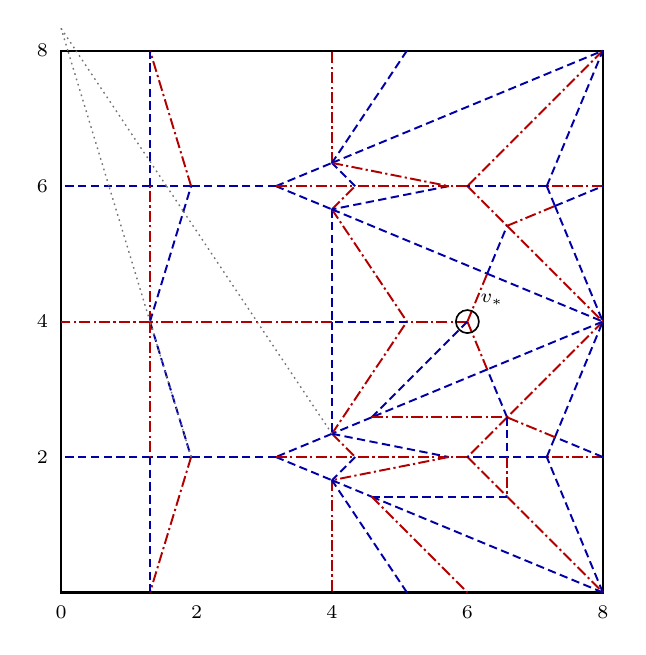
\begin{tikzpicture}[x=0.86cm,y=0.86cm]
\draw[sheet] (0,0) rectangle (8,8);
\draw[mtn] (8,6) -- (7.172,6);
\draw[mtn] (8,2) -- (7.172,2);
\draw[mtn] (6,2) -- (6.586,1.414);
\draw[mtn] (6,2) -- (5.725,2);
\draw[mtn] (8,4) -- (6.586,2.586);
\draw[mtn] (6,6) -- (6.586,5.414);
\draw[mtn] (6,6) -- (5.725,6);
\draw[mtn] (8,8) -- (6,6);
\draw[val] (3.172,6) -- (4,6.343);
\draw[val] (3.172,6) -- (1.92,6);
\draw[val] (3.172,2) -- (4,1.657);
\draw[val] (3.172,2) -- (1.92,2);
\draw[val] (3.172,6) -- (4,5.657);
\draw[val] (7.172,2) -- (7.293,2.293);
\draw[val] (7.172,2) -- (6.586,2);
\draw[val] (8,0) -- (7.172,2);
\draw[val] (7.172,6) -- (7.293,5.707);
\draw[val] (7.172,6) -- (6,6);
\draw[val] (7.172,6) -- (8,8);
\draw[val] (4,6.343) -- (8,8);
\draw[val] (4,1.657) -- (4.586,1.414);
\draw[val] (4,2.343) -- (3.172,2);
\draw[mtn] (4,5.657) -- (4.343,6);
\draw[val] (4.343,6) -- (4,6.343);
\draw[mtn] (4,6.343) -- (4,8);
\draw[val] (4,5.657) -- (4,4);
\draw[mtn] (4,2.343) -- (4.343,2);
\draw[val] (4.343,2) -- (4,1.657);
\draw[mtn] (4,1.657) -- (4,0);
\draw[mtn] (3.172,2) -- (4.343,2);
\draw[mtn] (3.172,6) -- (4.343,6);
\draw[mtn] (4,2.343) -- (5.107,4);
\draw[mtn] (4,5.657) -- (5.107,4);
\draw[val] (5.107,4) -- (4,4);
\draw[val] (4,4) -- (4,2.343);
\draw[val] (8,4) -- (6.293,3.293);
\draw[val] (4,5.657) -- (6.293,4.707);
\draw[mtn] (4,4) -- (1.313,4);
\draw[val] (5.725,6) -- (4,5.657);
\draw[mtn] (5.725,6) -- (4.343,6);
\draw[mtn] (4,6.343) -- (5.725,6);
\draw[val] (5.107,8) -- (4,6.343);
\draw[mtn] (5.725,2) -- (4.343,2);
\draw[val] (4,2.343) -- (5.725,2);
\draw[mtn] (5.725,2) -- (4,1.657);
\draw[val] (5.107,0) -- (4,1.657);
\draw[val] (1.313,4) -- (1.92,2);
\draw[val] (1.92,2) -- (1.313,2);
\draw[mtn] (1.313,4) -- (0,4);
\draw[mtn] (1.92,2) -- (1.313,0);
\draw[val] (1.92,6) -- (1.313,6);
\draw[mtn] (1.92,6) -- (1.313,8);
\draw[val] (1.313,2) -- (0,2);
\draw[val] (1.313,6) -- (0,6);
\draw[mtn] (1.313,4) -- (1.313,6);
\draw[val] (1.313,6) -- (1.313,8);
\draw[mtn] (1.313,4) -- (1.313,2);
\draw[val] (1.313,2) -- (1.313,0);
\draw[val] (7.293,2.293) -- (8,4);
\draw[val] (8,2) -- (7.293,2.293);
\draw[mtn] (7.293,2.293) -- (6.586,2.586);
\draw[mtn] (6.586,2.586) -- (6,2);
\draw[val] (6.586,2.586) -- (6.293,3.293);
\draw[val] (6.293,3.293) -- (4.586,2.586);
\draw[mtn] (6.293,3.293) -- (6,4);
\draw[mtn] (6,4) -- (5.107,4);
\draw[mtn] (6,4) -- (6.293,4.707);
\draw[val] (6.293,4.707) -- (8,4);
\draw[val] (6.293,4.707) -- (6.586,5.414);
\draw[mtn] (6.586,5.414) -- (8,4);
\draw[mtn] (6.586,5.414) -- (7.293,5.707);
\draw[val] (7.293,5.707) -- (8,4);
\draw[val] (7.293,5.707) -- (8,6);
\draw[val] (4.586,2.586) -- (4,2.343);
\draw[val] (6,4) -- (4.586,2.586);
\draw[mtn] (4.586,2.586) -- (6.586,2.586);
\draw[val] (6.586,2) -- (6,2);
\draw[val] (6.586,2.586) -- (6.586,2);
\draw[mtn] (6.586,2) -- (6.586,1.414);
\draw[mtn] (6.586,1.414) -- (8,0);
\draw[val] (6.586,1.414) -- (4.586,1.414);
\draw[val] (4.586,1.414) -- (8,0);
\draw[mtn] (4.586,1.414) -- (6,0);
\draw[val] (1.313,4) -- (1.92,6);
\draw[refl] (4,2.343) -- (2.893,4);
\draw[refl] (0,8.33) -- (0.22,8);
\draw[refl] (0.22,8) -- (1.313,6.364);
\draw[refl] (1.557,6) -- (1.807,5.626);
\draw[refl] (1.92,2) -- (1.313,4);
\draw[refl] (0.1,8) -- (0,8.33);
\draw[refl] (0.707,6) -- (0.1,8);
\draw[refl] (1.313,4) -- (0.707,6);
\draw[refl] (1.807,5.626) -- (2.893,4);
\draw[refl] (1.313,6.364) -- (1.557,6);
\draw[line width=0.6pt] (6,4) circle (0.17);
\node[font=\scriptsize,anchor=south west] at (6.05,4.1) {$\vstar$};
\foreach \x in {0,2,4,6,8} \node[font=\scriptsize,below] at (\x,-0.05) {$\x$};
\foreach \y in {2,4,6,8} \node[font=\scriptsize,left] at (-0.05,\y) {$\y$};
\end{tikzpicture}
\hspace{0.6em}
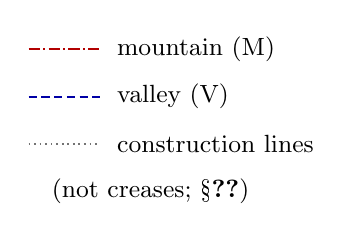
\begin{tikzpicture}[x=1cm,y=1cm,font=\small]
\draw[mtn] (0,2.2)--(0.9,2.2); \node[anchor=west] at (1,2.2) {mountain (M)};
\draw[val] (0,1.6)--(0.9,1.6); \node[anchor=west] at (1,1.6) {valley (V)};
\draw[refl] (0,1.0)--(0.9,1.0); \node[anchor=west] at (1,1.0) {construction lines};
\node[anchor=west,align=left] at (0,0.4) {\phantom{x}(not creases; \S\ref{sec:angles})};
\end{tikzpicture}
\caption{The crease pattern studied in this note, drawn on the square $Q=[0,8]^2$. It has $84$ creases and $32$ interior vertices. The circled vertex $\vstar=(6,4)$ is the one where a crease appears to stop for no reason; Section~\ref{sec:defect} explains it.}
\label{fig:cp}
\end{figure}

\section{Folding, reflection and cancellation}\label{sec:folding}

\begin{definition}
A \emph{crease pattern} on the square $Q=[0,8]^2$ is a finite set of closed segments in $Q$ (the \emph{creases}) that meet only at endpoints, each labelled M or V. The endpoints are \emph{vertices}; a vertex is \emph{interior} if it lies in the interior of $Q$ and a \emph{boundary vertex} otherwise. The creases divide $Q$ into convex polygons called \emph{faces}.
\end{definition}

Until Section~\ref{sec:deer}, which uses one physical fact, we need only the geometric shadow of folding, not the physical stacking of layers.

\begin{definition}
A \emph{flat folded state} of a crease pattern is a continuous map $f\colon Q\to\mathbb{R}^2$ that is an isometry on each face, such that for any two faces $F,F'$ sharing a crease $e$,
\begin{equation}\label{eq:adjacent}
f|_{F'} = f|_F\circ\rho_e ,
\end{equation}
where $\rho_e$ is the reflection of the plane in the line through $e$.
\end{definition}

Equation~\eqref{eq:adjacent} says that the paper turns over at every crease. A new fold is made along a line $\ell$ in the plane of the folded paper: some set $\mathcal M$ of faces (the layers that move) is replaced by its mirror image, $f'=\rho_\ell\circ f$ on $\mathcal M$ and $f'=f$ elsewhere, after first cutting faces along $f^{-1}(\ell)$ where necessary. The new creases lie in $f^{-1}(\ell)$. Two consequences of~\eqref{eq:adjacent} drive everything that follows.

\begin{lemma}[Reflection]\label{lem:reflection}
Let $F,F'$ be faces sharing a crease $e$, and suppose a fold along $\ell$ makes new creases in both $F$ and $F'$. Then inside $F\cup F'$ these new creases are mirror images of each other in the line of $e$.
\end{lemma}
\begin{proof}
The new crease in $F'$ lies in $(f|_{F'})^{-1}(\ell)=(f|_F\circ\rho_e)^{-1}(\ell)=\rho_e\bigl((f|_F)^{-1}(\ell)\bigr)$, the mirror image of the line containing the new crease in $F$.
\end{proof}

So a fold made after crease $e$, and passing through the layers on both sides of $e$, leaves a crease that \emph{bends} at $e$, with the two sides mirror images in $e$. Inside a single face it is straight. Its creases therefore form polygonal paths that turn only by reflection across earlier creases.

\begin{lemma}[Cancellation]\label{lem:cancel}
Let $e$ be a crease between faces $F,F'$ with $f(e)\subset\ell$. If a fold along $\ell$ moves $F'$ but not $F$, then afterwards $e$ is no longer a crease.
\end{lemma}
\begin{proof}
Since $f|_F$ is an isometry carrying the line of $e$ onto $\ell$, $f|_F\circ\rho_e=\rho_\ell\circ f|_F$. Hence $f'|_{F'}=\rho_\ell\circ f|_{F'}=\rho_\ell\circ f|_F\circ\rho_e=f|_F\circ\rho_e\circ\rho_e=f|_F=f'|_F$, so~\eqref{eq:adjacent} no longer holds across $e$: the paper is flat there.
\end{proof}

A later fold that lands exactly on an earlier crease therefore erases it. The erased segment is invisible in the final pattern, but it is best thought of as carrying \emph{two} creases, one from each fold, that cancel. Our example contains exactly one such segment. The theory below finds it without being told where to look.

Two further consequences of continuity are used in Section~\ref{sec:deer}.

\begin{lemma}[Moving boundary]\label{lem:boundary}
Let $F,F'$ be faces sharing an edge $e$. If a fold along $\ell$ moves $F'$ but not $F$, then $f(e)\subset\ell$.
\end{lemma}
\begin{proof}
A point $x\in e$ ends at $f(x)$ as a point of $F$ and at $\rho_\ell(f(x))$ as a point of $F'$. Continuity forces $\rho_\ell(f(x))=f(x)$, that is, $f(x)\in\ell$.
\end{proof}

So, going around a vertex, the paper can switch between moving and staying only across a ray that lands on the fold line.

\begin{lemma}[First crease]\label{lem:first}
Suppose every move folds along a single line. Then at each interior vertex $v$ of the final pattern, either two creases are collinear or some crease through $v$ was cancelled.
\end{lemma}
\begin{proof}
Consider the first move that creases the paper at $v$. Before it, a neighbourhood of $v$ is a single flat face, and the fold line $\ell$ passes through $f(v)$, so $f^{-1}(\ell)$ meets the neighbourhood in a line through $v$. By Lemma~\ref{lem:boundary}, moving and staying paper near $v$ are separated only by this line, so one half of the neighbourhood moves and both halves of the line become creases. Later moves never shift a crease within the sheet; by Lemma~\ref{lem:cancel} they can only cancel it.
\end{proof}

\section{From geometry to \texorpdfstring{$\ZN$}{Z/64Z}}\label{sec:discrete}

\begin{observation}\label{obs:discrete}
Every crease in Figure~\ref{fig:cp} has direction an integer multiple of $\delta=\pi/32=5.625^\circ$. The largest deviation of a measured direction from the nearest multiple is $0.013^\circ$, more than four hundred times smaller than $\delta$; we treat the directions as exact.
\end{observation}

Table~\ref{tab:dirs} lists the line directions that occur. Most are multiples of $\pi/8=22.5^\circ$, but not all: eight creases have odd multiples of $\pi/16$ and four have odd multiples of $\pi/32$. Section~\ref{sec:angles} explains why the unit is a power of two.

\begin{table}[h]
\centering\small
\begin{tabular}{rrr}
\toprule
$k$ & degrees & creases\\
\midrule
0&0&23\\ 2&11.25&2\\ 4&22.5&8\\ 8&45&6\\ 10&56.25&2\\ 12&67.5&5\\ 13&73.125&2\\
\bottomrule
\end{tabular}\qquad
\begin{tabular}{rrr}
\toprule
$k$ & degrees & creases\\
\midrule
16&90&10\\ 19&106.875&2\\ 20&112.5&5\\ 22&123.75&2\\ 24&135&7\\ 28&157.5&8\\ 30&168.75&2\\
\bottomrule
\end{tabular}
\caption{Line directions $k$ (in units of $\delta=\pi/32$, modulo $32$) occurring in the example, with the number of creases in each. Directions $2,10,22,30$ (odd multiples of $\pi/16$) and $13,19$ (odd multiples of $\pi/32$) each belong to a single chain (Section~\ref{sec:solve}).}
\label{tab:dirs}
\end{table}

A \emph{half-edge} is a pair $h=(v,e)$ with $v$ an endpoint of the crease $e$. Its \emph{direction} $d(h)\in\ZN$ is the direction of $e$ leaving $v$, in units of $\delta$, measured counterclockwise from the positive $x$-axis. A full turn is $64$, so the opposite direction of $x$ is $x+32$, and the line through a half-edge has direction $d(h)\bmod 32$. Write $H_v$ for the set of half-edges at $v$ and $D_v$ for the multiset of their directions.

Two maps on $\ZN$ express Lemma~\ref{lem:reflection}:
\begin{equation}\label{eq:maps}
\tau(x)=x+32 \quad\text{(continue straight)}, \qquad \sigma_c(x)=2c-x \quad\text{(reflect in a line of direction $c$)}.
\end{equation}
Both are involutions, and $\sigma_c=\sigma_{c+32}$, so $\sigma_c$ depends only on $c\bmod 32$. The only coincidence between them is the perpendicular one:
\begin{equation}\label{eq:perp}
\sigma_c(x)=\tau(x)\iff 2(c-x)\equiv 32 \pmod{64}\iff c\equiv x+16\pmod{32}.
\end{equation}
In words: a crease that crosses another at right angles looks the same whether or not it was reflected there. This is the one place where directions alone cannot tell us which fold came first.

From here on, the geometry enters only through incidence, meaning which half-edges share a vertex and which two form one crease. The one exception is a single ray we trace in Section~\ref{sec:defect}.

\section{The constraint problem}\label{sec:csp}

Lemma~\ref{lem:reflection} says that a chain passing through a vertex enters and leaves it in a related pair of directions. We adopt the simplest version of this.

\begin{assumption}\label{ass:pairs}
Every chain meets every interior vertex it passes through in exactly two half-edges $h,h'$. These satisfy $d(h')=\tau(d(h))$, or $d(h')=\sigma_{d(g)}(d(h))$ for some other half-edge $g$ at the same vertex, called a \emph{witness}.
\end{assumption}

Assumption~\ref{ass:pairs} allows a bend across one crease at a time. A fold through a point where several earlier creases meet could in principle bend by a product of several reflections; nothing of that kind is needed here.

\begin{definition}[Pairing]
An \emph{admissible pair} at an interior vertex $v$ is an unordered pair $\{h,h'\}\subseteq H_v$ that is \emph{straight} ($d(h')=\tau d(h)$) or \emph{reflected}: $d(h')=\sigma_{d(g)}(d(h))\neq d(h)$ for some \emph{witness} $g\in H_v\setminus\{h,h'\}$. A \emph{pairing} at $v$ is a set of disjoint admissible pairs; it is \emph{perfect} if it covers $H_v$.
\end{definition}

Fix a pairing at every interior vertex. Join two creases whenever their half-edges are paired at some vertex. Every crease has two ends and each end is paired at most once, so the connected components are paths or cycles; these are the \emph{chains}. If the pairing is perfect at every interior vertex, every path-shaped chain begins and ends on the boundary of $Q$.

\begin{definition}[Basic order]
If $\{h,h'\}$ is a reflected pair with witness $g$ and is not straight (equivalently, by~\eqref{eq:perp}, $g$ is not perpendicular to $h$), then the chain of $g$ was made before the chain of $h$. We write $K(g)\prec K(h)$. The \emph{basic order} is the transitive closure of these relations. It must be acyclic.
\end{definition}

Perfect pairings need not exist, as the vertex $\vstar$ will show. A perfect pairing can also exist and still make the local order cyclic, as at two vertices in Section~\ref{sec:deer}. Lemma~\ref{lem:cancel} tells us what to allow in both cases.

\begin{definition}[Hidden pair]
A \emph{hidden pair} is a segment $s$ from an interior vertex $v$ in a direction $r\in\ZN$, ending at the first point where the ray meets a crease or the boundary. It carries two coincident creases $\bar s_1,\bar s_2$, each contributing a half-edge of direction $r$ at $v$, denoted $\bar r$. The two creases are meant to belong to different chains and to cancel as in Lemma~\ref{lem:cancel}.
\end{definition}

\begin{definition}[Resolution]
A \emph{resolution} of a crease pattern is a finite set of hidden pairs together with a pairing at every interior vertex, of real and hidden half-edges, such that
\begin{enumerate}
\item[(L)] every pair is admissible and every pairing is perfect;
\item[(O)] the basic order is acyclic.
\end{enumerate}
A resolution is \emph{minimal} if it uses as few hidden pairs as possible.
\end{definition}

In a resolution, every chain ends on the boundary or closes up. Condition (O) is global but cheap to check, by attempting a topological sort. Hidden pairs are the only place where new geometry is introduced, so minimality keeps the theory from inventing structure.

\section{Solving the example}\label{sec:solve}

\subsection{The local stage}

At each interior vertex we list the admissible pairs and search for perfect pairings. Because pairs and witnesses are defined by the equations~\eqref{eq:maps} in $\ZN$, this is a finite check, carried out for all $32$ vertices in Appendix~\ref{app:table}. Two examples show what happens.

\begin{example}[A crossing]\label{ex:deg4}
At $v=(6-2\sqrt2,\,6)\approx(3.172,6)$, $D_v=\{0,4,32,60\}$. The pair $\{0,32\}$ is straight. The pair $\{4,60\}$ is reflected with witness $0$ (or $32$), since $\sigma_0(4)=-4=60$. None of the other four pairs $\{0,4\}$, $\{0,60\}$, $\{4,32\}$, $\{32,60\}$ is straight, and a witness would need $2c\equiv 4,60,36,28\pmod{64}$, i.e.\ $c\equiv 2,30,18,14\pmod{32}$. No such half-edge exists, so the perfect pairing is unique: a horizontal chain passes straight through, and a second chain bends across it.
\end{example}

\begin{example}[Three chains through one point]\label{ex:deg6}
At $v=(4,\,8-4\sqrt2)\approx(4,2.343)$ the directions are $D_v=\{4,10,16,\allowbreak 36,56,62\}$, and the admissible pairs are
\[
\begin{gathered}
\{4,36\}\ \text{straight};\qquad \{16,56\},\ \{10,62\}\ \text{reflected, witness }4\text{ or }36;\\
\{4,16\}\ \text{reflected, witness }10;\qquad \{4,56\}\ \text{reflected, witness }62.
\end{gathered}
\]
The last two cannot be completed: after $\{4,16\}$ the remaining $10,36,56,62$ admit only $\{10,62\}$, which strands $36$ and $56$, and similarly after $\{4,56\}$. The unique perfect pairing is $\{4,36\}$, $\{16,56\}$, $\{10,62\}$: one chain passes straight through, and two others bend across it.
\end{example}

\begin{proposition}\label{prop:local}
At each of the $31$ interior vertices other than $\vstar=(6,4)$, the real half-edges have exactly one perfect pairing. At $\vstar$ they have no perfect pairing.
\end{proposition}
\begin{proof}
A finite computation (Appendix~\ref{app:table}). For $\vstar$, see below.
\end{proof}

\subsection{The defect vertex}\label{sec:defect}

At $\vstar=(6,4)$, $D_{\vstar}=\{12,32,40,52\}$ (Figure~\ref{fig:vstar}). The only admissible pair is $\{12,52\}$, which is reflected since $\sigma_0(12)=52$; its witness is the half-edge $32$. The half-edge $32$ belongs to the horizontal chain along $y=4$, which simply stops here. The half-edge $40$ has no admissible partner either. Checking all candidates, $\tau(32)=0$, $\sigma_{12}(32)=56$, $\sigma_{40}(32)=48$ and $\sigma_{52}(32)=8$, none of which is in $D_{\vstar}$, and similarly for $40$. So $\vstar$ has two unpaired half-edges.

\begin{proposition}\label{prop:defect}
Any resolution using a single hidden pair places it at $\vstar$ in direction $r=0$. The segment runs from $(6,4)$ to the boundary point $(8,4)$ and crosses no crease. In this resolution the horizontal chain continues straight, $\{32,\bar 0\}$, and the chain of $40$ bends across the witness $52$, $\{40,\bar 0\}$.
\end{proposition}
\begin{proof}
The half-edges $32$ and $40$ have no real partner at $\vstar$, and breaking up $\{12,52\}$ only adds unpaired half-edges. So each of $32$ and $40$ must be paired with a hidden half-edge at $\vstar$. With one hidden pair, these are its two copies $\bar r$, and $r$ must be admissible as a partner of both. The possible partners of $32$ at $\vstar$ are $\tau(32)=0$ and $\sigma_c(32)$ for $c\in\{12,40,52\}$, giving $\{0,56,48,8\}$. Those of $40$ are $\tau(40)=8$ and $\sigma_c(40)$ for $c\in\{12,32,52\}$, giving $\{8,48,24,0\}$. Hence $r\in\{0,8,48\}$. Write $A^0$ for the chain of $32$, $F$ for the chain of $40$, and $I$ for the chain of $\{12,52\}$, whose witness line, direction $0\bmod 32$, carries $A^0$ and possibly a hidden half-edge.
\begin{itemize}
\item $r=8$: $\{32,\bar 8\}$ is reflected only across $52$ (as $\sigma_{52}(32)=8$), giving $I\prec A^0$. The witness of $\{12,52\}$ must lie on the line $0\bmod 32$, which now carries only $A^0$, giving $A^0\prec I$. This is a cycle.
\item $r=48$: $\{32,\bar{48}\}$ is reflected across $40$, giving $F\prec A^0$. $\{40,\bar{48}\}$ is reflected across $12$, giving $I\prec F$. As before $A^0\prec I$. This is a cycle.
\item $r=0$: $\{32,\bar 0\}$ is straight. $\{40,\bar 0\}$ is reflected across $52$, as $\sigma_{52}(40)=64\equiv 0$, giving $I\prec F$. The witness of $\{12,52\}$ may be $A^0$ or the hidden half-edge of $F$. The latter gives $F\prec I$, a cycle, so the witness is $A^0$ and $A^0\prec I\prec F$. This is acyclic.
\end{itemize}
Finally, the ray from $(6,4)$ in direction $0$ meets no crease before the boundary point $(8,4)$. So the hidden creases end on the boundary and nothing else changes.
\end{proof}

Read as folding history, Proposition~\ref{prop:defect} says that the horizontal crease along $y=4$ originally ran to the edge. Later, $I$ was folded across it, and later still $F$ was folded across $I$ exactly along the image of that crease, erasing it as in Lemma~\ref{lem:cancel}. Nothing about $\vstar$ was assumed: the vertex was flagged because the local stage failed there, and acyclicity left one repair.

\begin{figure}[t]
\centering
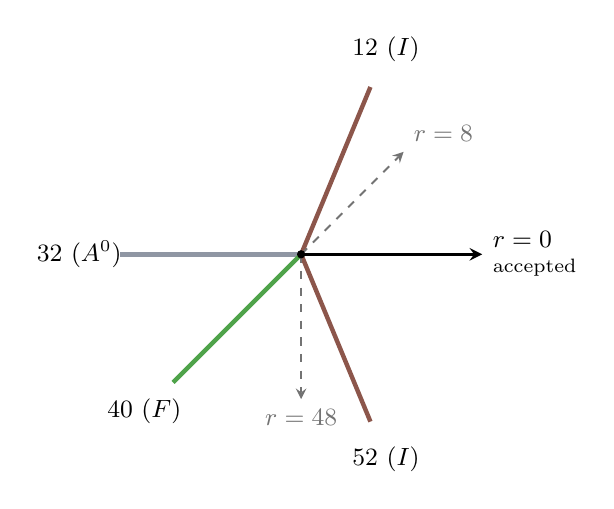
\begin{tikzpicture}[x=1.15cm,y=1.15cm,font=\small,>=stealth]
\foreach \d/\lab/\col in {12/{$12$ ($I$)}/cI, 52/{$52$ ($I$)}/cI, 32/{$32$ ($A^0$)}/cA, 40/{$40$ ($F$)}/cF}{
  \draw[line width=1.6pt,\col] (0,0) -- ({2*cos(\d*5.625)},{2*sin(\d*5.625)});
  \node at ({2.45*cos(\d*5.625)},{2.45*sin(\d*5.625)}) {\lab};}
\draw[->,line width=1pt,black] (0,0) -- (2,0) node[right,align=left] {$r=0$\\[-2pt]\scriptsize accepted};
\draw[->,line width=0.7pt,black!55,dashed] (0,0) -- ({1.6*cos(45)},{1.6*sin(45)}) node[above right] {$r=8$};
\draw[->,line width=0.7pt,black!55,dashed] (0,0) -- (0,-1.6) node[below] {$r=48$};
\fill (0,0) circle (1.5pt);
\end{tikzpicture}
\caption{The vertex $\vstar=(6,4)$. Solid: the four real half-edges with their directions in units of $\pi/32$. Arrows: the three directions in which a hidden pair could pair both $32$ and $40$. Only $r=0$ leaves the basic order acyclic.}
\label{fig:vstar}
\end{figure}

\subsection{Chains}

\begin{theorem}\label{thm:chains}
The crease pattern of Figure~\ref{fig:cp} has no resolution without hidden pairs, and exactly one with one hidden pair. It has $15$ chains, every one running from boundary to boundary (Figure~\ref{fig:chains}, Table~\ref{tab:chains}).
\end{theorem}
\begin{proof}
By Proposition~\ref{prop:local} the pairings at the other $31$ vertices are forced. By Proposition~\ref{prop:defect} so is the repair at $\vstar$. The hidden segment ends on the boundary, so it adds no constraint elsewhere. Following the pairings gives the $15$ chains, and condition (O) is verified in Section~\ref{sec:order}.
\end{proof}

We name the chains by where they lie. $A^{+},A^{0},A^{-}$ are the horizontal lines $y=6,4,2$. $P_i^{\pm}$ are the three pairs of chains at the right end of the sheet: $P_1^{\pm}$ at $22.5^\circ$, $P_2^{\pm}$ at $45^\circ$ and $P_3^{\pm}$ at $67.5^\circ$ from the bottom edge. $I$ (inner) and $F$ (flattening) meet at $\vstar$. $C,C'$ are the two chains near $x=4$, and $E,E'$ the two near $x=1.3$. Each $P_i^{+}$ is the mirror image of $P_i^{-}$ in the line $y=4$, as is $A^{+}$ of $A^{-}$. Chains related this way can be made by a single fold through a stack of layers, but deciding such groupings is beyond the basic theory.

\begin{figure}[t]
\centering
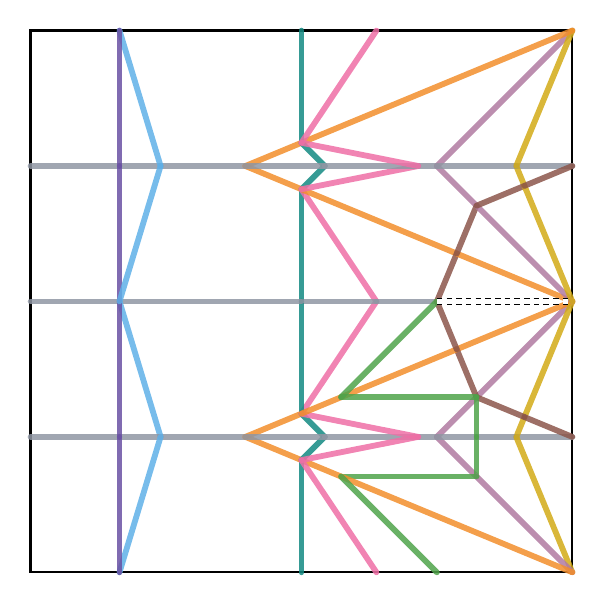
\begin{tikzpicture}[x=0.86cm,y=0.86cm]
\draw[sheet] (0,0) rectangle (8,8);
\draw[ch,cA] (8,6) -- (7.172,6);
\draw[ch,cA] (8,2) -- (7.172,2);
\draw[ch,cP2] (6,2) -- (6.586,1.414);
\draw[ch,cA] (6,2) -- (5.725,2);
\draw[ch,cP2] (8,4) -- (6.586,2.586);
\draw[ch,cP2] (6,6) -- (6.586,5.414);
\draw[ch,cA] (6,6) -- (5.725,6);
\draw[ch,cP2] (8,8) -- (6,6);
\draw[ch,cP1] (3.172,6) -- (4,6.343);
\draw[ch,cA] (3.172,6) -- (1.92,6);
\draw[ch,cP1] (3.172,2) -- (4,1.657);
\draw[ch,cA] (3.172,2) -- (1.92,2);
\draw[ch,cP1] (3.172,6) -- (4,5.657);
\draw[ch,cP3] (7.172,2) -- (7.293,2.293);
\draw[ch,cA] (7.172,2) -- (6.586,2);
\draw[ch,cP3] (8,0) -- (7.172,2);
\draw[ch,cP3] (7.172,6) -- (7.293,5.707);
\draw[ch,cA] (7.172,6) -- (6,6);
\draw[ch,cP3] (7.172,6) -- (8,8);
\draw[ch,cP1] (4,6.343) -- (8,8);
\draw[ch,cP1] (4,1.657) -- (4.586,1.414);
\draw[ch,cP1] (4,2.343) -- (3.172,2);
\draw[ch,cC] (4,5.657) -- (4.343,6);
\draw[ch,cC] (4.343,6) -- (4,6.343);
\draw[ch,cC] (4,6.343) -- (4,8);
\draw[ch,cC] (4,5.657) -- (4,4);
\draw[ch,cC] (4,2.343) -- (4.343,2);
\draw[ch,cC] (4.343,2) -- (4,1.657);
\draw[ch,cC] (4,1.657) -- (4,0);
\draw[ch,cA] (3.172,2) -- (4.343,2);
\draw[ch,cA] (3.172,6) -- (4.343,6);
\draw[ch,cCp] (4,2.343) -- (5.107,4);
\draw[ch,cCp] (4,5.657) -- (5.107,4);
\draw[ch,cA] (5.107,4) -- (4,4);
\draw[ch,cC] (4,4) -- (4,2.343);
\draw[ch,cP1] (8,4) -- (6.293,3.293);
\draw[ch,cP1] (4,5.657) -- (6.293,4.707);
\draw[ch,cA] (4,4) -- (1.313,4);
\draw[ch,cCp] (5.725,6) -- (4,5.657);
\draw[ch,cA] (5.725,6) -- (4.343,6);
\draw[ch,cCp] (4,6.343) -- (5.725,6);
\draw[ch,cCp] (5.107,8) -- (4,6.343);
\draw[ch,cA] (5.725,2) -- (4.343,2);
\draw[ch,cCp] (4,2.343) -- (5.725,2);
\draw[ch,cCp] (5.725,2) -- (4,1.657);
\draw[ch,cCp] (5.107,0) -- (4,1.657);
\draw[ch,cEp] (1.313,4) -- (1.92,2);
\draw[ch,cA] (1.92,2) -- (1.313,2);
\draw[ch,cA] (1.313,4) -- (0,4);
\draw[ch,cEp] (1.92,2) -- (1.313,0);
\draw[ch,cA] (1.92,6) -- (1.313,6);
\draw[ch,cEp] (1.92,6) -- (1.313,8);
\draw[ch,cA] (1.313,2) -- (0,2);
\draw[ch,cA] (1.313,6) -- (0,6);
\draw[ch,cE] (1.313,4) -- (1.313,6);
\draw[ch,cE] (1.313,6) -- (1.313,8);
\draw[ch,cE] (1.313,4) -- (1.313,2);
\draw[ch,cE] (1.313,2) -- (1.313,0);
\draw[ch,cP3] (7.293,2.293) -- (8,4);
\draw[ch,cI] (8,2) -- (7.293,2.293);
\draw[ch,cI] (7.293,2.293) -- (6.586,2.586);
\draw[ch,cP2] (6.586,2.586) -- (6,2);
\draw[ch,cI] (6.586,2.586) -- (6.293,3.293);
\draw[ch,cP1] (6.293,3.293) -- (4.586,2.586);
\draw[ch,cI] (6.293,3.293) -- (6,4);
\draw[ch,cA] (6,4) -- (5.107,4);
\draw[ch,cI] (6,4) -- (6.293,4.707);
\draw[ch,cP1] (6.293,4.707) -- (8,4);
\draw[ch,cI] (6.293,4.707) -- (6.586,5.414);
\draw[ch,cP2] (6.586,5.414) -- (8,4);
\draw[ch,cI] (6.586,5.414) -- (7.293,5.707);
\draw[ch,cP3] (7.293,5.707) -- (8,4);
\draw[ch,cI] (7.293,5.707) -- (8,6);
\draw[ch,cP1] (4.586,2.586) -- (4,2.343);
\draw[ch,cF] (6,4) -- (4.586,2.586);
\draw[ch,cF] (4.586,2.586) -- (6.586,2.586);
\draw[ch,cA] (6.586,2) -- (6,2);
\draw[ch,cF] (6.586,2.586) -- (6.586,2);
\draw[ch,cF] (6.586,2) -- (6.586,1.414);
\draw[ch,cP2] (6.586,1.414) -- (8,0);
\draw[ch,cF] (6.586,1.414) -- (4.586,1.414);
\draw[ch,cP1] (4.586,1.414) -- (8,0);
\draw[ch,cF] (4.586,1.414) -- (6,0);
\draw[ch,cEp] (1.313,4) -- (1.92,6);
\draw[virt] (6,4) -- (8,4);
\end{tikzpicture}
\hspace{0.8em}
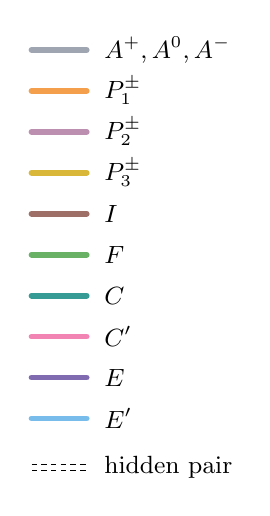
\begin{tikzpicture}[x=1cm,y=0.52cm,font=\small]
\foreach \c/\n [count=\i] in {cA/{$A^{+},A^{0},A^{-}$},cP1/{$P_1^{\pm}$},cP2/{$P_2^{\pm}$},cP3/{$P_3^{\pm}$},cI/{$I$},cF/{$F$},cC/{$C$},cCp/{$C'$},cE/{$E$},cEp/{$E'$}}{
  \draw[ch,\c] (0,-\i)--(0.7,-\i); \node[anchor=west] at (0.8,-\i) {\n};}
\draw[virt] (0,-11.2)--(0.7,-11.2); \node[anchor=west] at (0.8,-11.2) {hidden pair};
\end{tikzpicture}
\caption{The $15$ chains, coloured by family; a superscript $+$ marks the upper member of a mirror pair. The double dotted segment from $\vstar=(6,4)$ to $(8,4)$ is the hidden pair of Proposition~\ref{prop:defect}: one of its creases belongs to $A^0$, the other to $F$.}
\label{fig:chains}
\end{figure}

\begin{table}[t]
\centering\footnotesize\setlength{\tabcolsep}{4pt}
\begin{tabular}{lcllll}
\toprule
chain & creases & from $\to$ to & colours & bends across & crosses at right angles\\
\midrule
$A^{+}$ & 8 & $(0,6)\to(8,6)$ & \texttt{VVVMMMVM} & -- & $E$\\
$A^{0}$ & 5 & $(0,4)\to(8,4)$ & \texttt{MMVM0} & -- & $C$, $E$\\
$A^{-}$ & 9 & $(0,2)\to(8,2)$ & \texttt{VVVMMMVVM} & -- & $E$, $F$\\
$P_1^{+}$ & 5 & $(8,4)\to(8,8)$ & \texttt{VVVVV} & $A^{+}$ & $I$\\
$P_1^{-}$ & 7 & $(8,0)\to(8,4)$ & \texttt{VVVVVVV} & $A^{-}$ & $I$\\
$P_2^{+}$ & 3 & $(8,4)\to(8,8)$ & \texttt{MMM} & $A^{+}$ & --\\
$P_2^{-}$ & 4 & $(8,0)\to(8,4)$ & \texttt{MMMM} & $A^{-}$ & --\\
$P_3^{+}$ & 3 & $(8,4)\to(8,8)$ & \texttt{VVV} & $A^{+}$ & $I$\\
$P_3^{-}$ & 3 & $(8,0)\to(8,4)$ & \texttt{VVV} & $A^{-}$ & $I$\\
$I$ & 8 & $(8,2)\to(8,6)$ & \texttt{VMVMMVMV} & $P_2^{-}$, $P_2^{+}$, $A^{0}$ & $P_1^{+}$, $P_1^{-}$, $P_3^{-}$, $P_3^{+}$\\
$F$ & 7 & $(6,0)\to(8,4)$ & \texttt{MVMVMV0} & $P_2^{-}$, $P_1^{-}$, $I$ & $A^{-}$\\
$C$ & 8 & $(4,0)\to(4,8)$ & \texttt{MVMVVMVM} & $A^{+}$, $A^{-}$, $P_1^{+}$, $P_1^{-}$ & $A^{0}$\\
$C'$ & 8 & $(5.107,0)\to(5.107,8)$ & \texttt{VMVMMVMV} & $A^{+}$, $A^{-}$, $P_1^{+}$, $P_1^{-}$, $A^{0}$ & --\\
$E$ & 4 & $(1.313,0)\to(1.313,8)$ & \texttt{VMMV} & -- & $A^{+}$, $A^{-}$, $A^{0}$\\
$E'$ & 4 & $(1.313,0)\to(1.313,8)$ & \texttt{MVVM} & $A^{+}$, $A^{-}$, $A^{0}$ & --\\
\bottomrule
\end{tabular}
\caption{The chains. ``Colours'' lists M/V along the chain from the first endpoint to the second; \texttt{0} marks the hidden crease. ``Bends across'' lists the witnesses of reflected, non-perpendicular pairs, which are the generators of the basic order. The last column lists right-angle crossings, which the basic order ignores~\eqref{eq:perp}.}
\label{tab:chains}
\end{table}

\subsection{The basic order}\label{sec:order}

Reading off the witnesses (Table~\ref{tab:chains}) gives $24$ relations, and they are acyclic. Their transitive reduction has the $19$ edges shown in Figure~\ref{fig:hasse}.

\begin{corollary}\label{cor:order}
The basic order on the $15$ chains is the partial order of Figure~\ref{fig:hasse}. In particular:
\begin{enumerate}
\item the three horizontal chains are minimal;
\item $A^{0}\prec I\prec F$, and $F$ also follows $P_1^{-}$ and $P_2^{-}$;
\item $C$ and $C'$ follow $A^{\pm}$ and $P_1^{\pm}$ ($C'$ also follows $A^0$), but are incomparable with $I$, $F$, $P_2^\pm$ and $P_3^\pm$;
\item $E$ is incomparable with every other chain.
\end{enumerate}
The basic order has $172{,}768{,}020$ linear extensions.
\end{corollary}

Item 4 is instructive. $E$ is the vertical line $x=8\sqrt2-10\approx1.313$, and it meets other creases only at right angles, so by the perpendicular coincidence~\eqref{eq:perp} reflection says nothing about it. The large number of linear extensions is mostly due to chains like this, and to independent groups such as $\{C,C'\}$ versus $\{I,F\}$. Narrowing it down needs rules outside the basic theory, beginning with colour.

\begin{figure}[t]
\centering
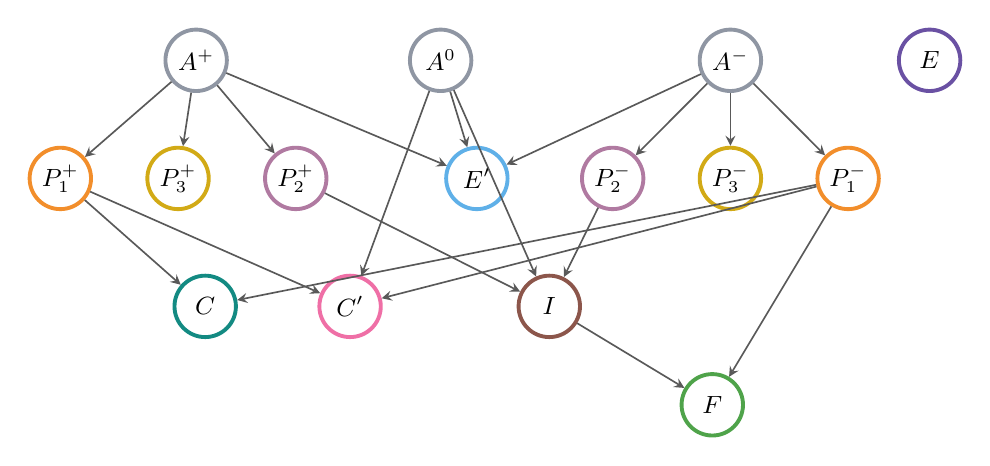
\begin{tikzpicture}[x=1.15cm,y=1.25cm,font=\small,>=stealth,
  nd/.style={circle,inner sep=1.2pt,minimum size=0.78cm,line width=1.4pt,fill=white}]
\node[nd,draw=cA] (Ap) at (1.5,3) {$A^{+}$};
\node[nd,draw=cA] (A0) at (4.2,3) {$A^{0}$};
\node[nd,draw=cA] (Am) at (7.4,3) {$A^{-}$};
\node[nd,draw=cE] (E) at (9.6,3) {$E$};
\node[nd,draw=cP1] (P1p) at (0,1.8) {$P_1^{+}$};
\node[nd,draw=cP3] (P3p) at (1.3,1.8) {$P_3^{+}$};
\node[nd,draw=cP2] (P2p) at (2.6,1.8) {$P_2^{+}$};
\node[nd,draw=cEp] (Ep) at (4.6,1.8) {$E'$};
\node[nd,draw=cP2] (P2m) at (6.1,1.8) {$P_2^{-}$};
\node[nd,draw=cP3] (P3m) at (7.4,1.8) {$P_3^{-}$};
\node[nd,draw=cP1] (P1m) at (8.7,1.8) {$P_1^{-}$};
\node[nd,draw=cC] (C) at (1.6,0.5) {$C$};
\node[nd,draw=cCp] (Cp) at (3.2,0.5) {$C'$};
\node[nd,draw=cI] (I) at (5.4,0.5) {$I$};
\node[nd,draw=cF] (F) at (7.2,-0.5) {$F$};
\foreach \a/\b in {Ap/P2p,Ap/P1p,Ap/P3p,Ap/Ep,Am/P2m,Am/P1m,Am/P3m,Am/Ep,A0/Cp,A0/Ep,A0/I,P2m/I,P2p/I,P1p/C,P1p/Cp,P1m/C,P1m/Cp,P1m/F,I/F}
  \draw[->,line width=0.6pt,black!65] (\a) -- (\b);
\end{tikzpicture}
\caption{Hasse diagram of the basic order: an arrow $K\to K'$ means $K\prec K'$, i.e.\ $K$ was made first.}
\label{fig:hasse}
\end{figure}

\section{What colour adds}\label{sec:colour}

Nothing above used the labels M and V, and the chains were identified without them. Colour enters through Maekawa's theorem: at an interior vertex of a flat-foldable pattern, the numbers of mountain and valley creases differ by exactly $2$~\cite{hull}. At a vertex of degree four where chain $Y$ bends across a straight chain $X$, the four colours are those of $X$'s two creases and $Y$'s two creases. Maekawa's theorem then forces exactly one of the two chains to change colour at the vertex. Which one is recorded in the pattern, and Table~\ref{tab:chains} shows two regimes.
\begin{itemize}
\item \emph{$Y$ changes colour and $X$ does not.} This happens for $C$, $C'$ and $E'$ bending across $A^{\pm}$, $I$ across $P_2^+$, and $F$ across $P_1^-$ and $P_2^-$. It is what folding $Y$ produces when the layers on both sides of $X$ turn the same way.
\item \emph{$Y$ keeps its colour and $X$ changes.} This happens for every $P_i^{\pm}$ across $A^{\pm}$, and for $C'$ across $A^0$. Here the layers on the two sides of $X$ turn in opposite directions, and the part of $X$ beyond $Y$ is turned over; origami calls this a \emph{reverse fold}. Thus $A^{+}$ changes colour exactly where $P_1^+$, $P_2^+$ and $P_3^+$ cross it. At $(8\sqrt2-10,\,4)$, where $E$ and $E'$ both cross $A^0$, both keep their colour and $A^0$ does not change, as if two such changes cancelled.
\end{itemize}

Colour also gives a consistency check on the hidden pair. At $\vstar$, $I$ keeps its colour (M,M) across $A^0$, so by the second regime the hidden continuation of $A^0$ (M before $\vstar$) is V. $F$ changes colour at every one of its other bends, and continuing that pattern makes its hidden crease M, opposite to its V crease at $\vstar$. A valley and a mountain on one segment are exactly the cancelling pair of Lemma~\ref{lem:cancel}. This is a check, not a derivation: turning such regimes into ordering rules belongs to the more complex theory we set aside.

Colour does not settle right-angle crossings by itself. Maekawa's theorem still says that one chain changes colour there, but either the later chain changed colour or the earlier one was turned over. The chain $E$ shows the gap. Its colours V, M, M, V tell us it is not the first fold, since a single fold of a flat sheet has one colour, but not which fold preceded it.

\section{Where the angles come from}\label{sec:angles}

Why should every direction be a multiple of $\pi/32$, and why do the finer directions occur only in $C'$ and $E'$? In this pattern, folds are placed by bisecting angles, and each bisection can halve the angular unit.
\begin{itemize}
\item At the vertex of Example~\ref{ex:deg6}, $C'$ has direction $10=\tfrac12(16+4)$. It bisects the angle between $C$ (direction $16$) and $P_1^{-}$ (direction $4$). This is how odd multiples of $\pi/16$ arise.
\item The dotted construction line in Figure~\ref{fig:cp} leaves that vertex in direction $22=\sigma_{16}(10)$. This is where $C'$ lands once the paper is folded along $C$; in the folded model it is a visible folded edge. The crease $E'$, of direction $19=\tfrac12(16+22)$, bisects the angle between this line and the left edge of the sheet (direction $16$). The second dotted line extends $E'$, and all three lines meet at one point on the extension of the left edge, as a bisector must. This is how odd multiples of $\pi/32$ arise.
\end{itemize}
In folding terms, $E'$ is placed by laying the end of the folded strip along the folded edge left by the crimp $C,C'$. Its reference is itself a bisector, which is why its direction needs the finest unit in the pattern. For identifying chains, though, only the integrality of directions matters, and that holds whatever its origin.

\section{A second example: when the order is not enough}\label{sec:deer}

Figure~\ref{fig:deer} shows a smaller pattern, the body of a four-legged animal. It has 15 creases and five interior vertices: the centre $c=(4,4)$, the points $p_\pm=(4,4\pm2)$ on the central vertical crease, and the points $q_\pm=(2,4\pm2)$ on the left edge of the rectangle. Every direction is a multiple of $\pi/4$, so $N=8$; in this section directions are in units of $\pi/4$, lines are taken modulo $4$, and $\tau(x)=x+4$.

\begin{figure}[t]
\centering
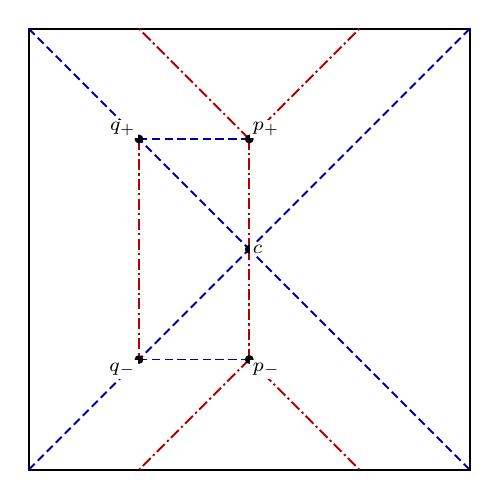
\begin{tikzpicture}[x=0.7cm,y=0.7cm]
\draw[sheet] (0,0) rectangle (8,8);
\draw[mtn] (4,4)--(4,6); \draw[mtn] (4,4)--(4,2); \draw[mtn] (2,6)--(2,2);
\draw[mtn] (4,2)--(2,0); \draw[mtn] (4,2)--(6,0); \draw[mtn] (4,6)--(2,8); \draw[mtn] (4,6)--(6,8);
\draw[val] (0,0)--(4,4); \draw[val] (0,8)--(4,4); \draw[val] (8,8)--(4,4); \draw[val] (8,0)--(4,4);
\draw[val] (4,2)--(2,2); \draw[val] (4,6)--(2,6);
\foreach \p/\n/\a in {(4,4)/c/west, (4,6)/p_+/south west, (4,2)/p_-/north west, (2,6)/q_+/south east, (2,2)/q_-/north east}
  {\fill \p circle (1.6pt); \node[font=\scriptsize,anchor=\a,fill=white,inner sep=1pt] at \p {$\n$};}
\end{tikzpicture}
\caption{The second pattern, rescaled to $Q=[0,8]^2$, drawn with the same conventions as Figure~\ref{fig:cp}.}
\label{fig:deer}
\end{figure}

\subsection{Resolutions}

The local stage runs exactly as in Section~\ref{sec:solve}; Table~\ref{tab:deer} gives the result.

\begin{table}[h]
\centering\small
\begin{tabular}{llll}
\toprule
vertex & $D_v$ & perfect pairings & status\\
\midrule
$q_+=(2,6)$ & $0,3,6,7$ & $\{3,7\}\,\tau$; $\{0,6\}\,\sigma_3$ & forced\\
$q_-=(2,2)$ & $0,1,2,5$ & $\{1,5\}\,\tau$; $\{0,2\}\,\sigma_1$ & forced\\
$c=(4,4)$ & $1,2,3,5,6,7$ & A: $\{2,6\}\,\tau$; $\{1,3\}\,\sigma_2$; $\{5,7\}\,\sigma_2$ & two pairings,\\
 & & B: $\{2,6\}\,\tau$; $\{1,5\}\,\tau$; $\{3,7\}\,\tau$ & both acyclic\\
$p_+=(4,6)$ & $1,3,4,6$ & $\{1,3\}\,\sigma_2$; $\{4,6\}\,\sigma_1$ & locally cyclic\\
$p_-=(4,2)$ & $2,4,5,7$ & $\{5,7\}\,\sigma_2$; $\{2,4\}\,\sigma_3$ & locally cyclic\\
\bottomrule
\end{tabular}
\caption{The local stage for the second pattern. At $p_\pm$ the only perfect pairing makes two chains bend across each other.}
\label{tab:deer}
\end{table}

At $p_+$ the only perfect pairing joins the vertical crease to the top edge of the rectangle, and the resulting chain and the small V each bend across the other. The local order is therefore cyclic, so condition (O) fails without hidden pairs. This is no accident. A perfect pairing with no straight pair is always locally cyclic: each chain at the vertex bends across another chain there, so the local order has no first element. By Lemma~\ref{lem:first}, a vertex without a collinear pair needs a cancelled crease, unless it was made by a move that is not a single-line fold.

One hidden pair at each of $p_\pm$ repairs this. At $p_+$ two directions keep the local order acyclic. One continues the vertical crease up to the edge at $(4,8)$, crossing nothing. The other runs diagonally into the sheet and stops at the first crease it meets, where its two hidden creases have nothing to pair with, so it yields no resolution. With the first, the vertical continues straight, the rectangle's top edge turns up across the small V, and the order there is vertical $\prec$ small V $\prec$ rectangle. The same happens at $p_-$, downwards. Writing $X$ for the vertical, $R$ for the rectangle chain (whose two ends are the hidden creases beside $X$'s), and $U,L$ for the small V's, the remaining choice is at $c$.

\begin{proposition}\label{prop:deer}
The second pattern has exactly two minimal resolutions, each with one hidden pair at $p_+$ and one at $p_-$ (Figure~\ref{fig:deerres}).
\begin{itemize}
\item In \emph{A}, the big diagonals bend across $X$ at $c$, forming two V-shaped chains: $V^+$ from $(0,8)$ through $c$ to $(8,8)$, and $V^-$ from $(0,0)$ through $c$ to $(8,0)$. The order is generated by $X\prec U,L,V^\pm$ and $U,L,V^\pm\prec R$.
\item In \emph{B}, all three lines pass straight through $c$, as diagonals $D_1$ from $(0,0)$ to $(8,8)$ and $D_2$ from $(0,8)$ to $(8,0)$. The order is generated by $X\prec U,L$ and $U,L,D_1,D_2\prec R$.
\end{itemize}
Both orders are acyclic, so the basic theory cannot choose.
\end{proposition}

\begin{figure}[t]
\centering
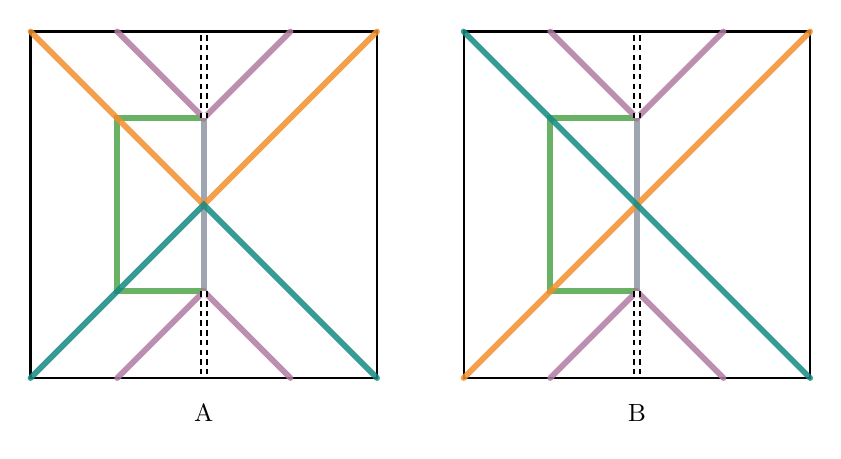
\begin{tikzpicture}[x=0.55cm,y=0.55cm]
\begin{scope}
\draw[sheet] (0,0) rectangle (8,8);
\draw[ch,cA] (4,2)--(4,6);
\draw[ch,cF] (4,6)--(2,6)--(2,2)--(4,2);
\draw[ch,cP2] (2,8)--(4,6)--(6,8); \draw[ch,cP2] (2,0)--(4,2)--(6,0);
\draw[ch,cP1] (0,8)--(4,4)--(8,8);
\draw[ch,cC] (0,0)--(4,4)--(8,0);
\draw[virt] (4,6)--(4,8); \draw[virt] (4,2)--(4,0);
\node[font=\small] at (4,-0.8) {A};
\end{scope}
\begin{scope}[xshift=5.5cm]
\draw[sheet] (0,0) rectangle (8,8);
\draw[ch,cA] (4,2)--(4,6);
\draw[ch,cF] (4,6)--(2,6)--(2,2)--(4,2);
\draw[ch,cP2] (2,8)--(4,6)--(6,8); \draw[ch,cP2] (2,0)--(4,2)--(6,0);
\draw[ch,cP1] (0,0)--(8,8);
\draw[ch,cC] (0,8)--(8,0);
\draw[virt] (4,6)--(4,8); \draw[virt] (4,2)--(4,0);
\node[font=\small] at (4,-0.8) {B};
\end{scope}
\end{tikzpicture}
\caption{The two resolutions of Proposition~\ref{prop:deer}. Grey: $X$; green: $R$; mauve: $U$ and $L$; orange and teal: $V^+$ and $V^-$ in A, $D_1$ and $D_2$ in B. The double dotted segments are the hidden pairs, each shared by $X$ and $R$.}
\label{fig:deerres}
\end{figure}

\subsection{Ruling out B}

To go further we need the physical model behind Section~\ref{sec:folding}. We assume each move folds the paper along \emph{one} line $\ell$: some of the paper turns over about $\ell$ and the rest stays. Unfolding is allowed, since it is itself such a move. We read each chain as the set of creases last set by one move, which is the fold that made them unless they were later unfolded and refolded. The one physical fact we add is that the turning paper rotates by a half-turn about $\ell$, and paper cannot pass through paper.

\begin{proposition}\label{prop:notB}
No sequence of single-line moves produces resolution B. Resolution A passes the same test.
\end{proposition}

\begin{proof}
Suppose a sequence produces B. The argument has four steps, all at $c$.

\emph{1. The last of the three lines is the vertical, folded over both diagonals.} Consider the last move that sets a crease at $c$. In B each of the three lines through $c$ is a chain of its own, so this move sets exactly one line. Just before it, the other two lines are folded at $c$ and this one is flat. That earlier state is flat-folded, so it satisfies Kawasaki's condition at $c$: alternate angles around $c$ sum to $\pi$~\cite{hull}. With the vertical and one diagonal folded, the angles around $c$ are $45^\circ,135^\circ,45^\circ,135^\circ$, and their alternate sums are $90^\circ$ and $270^\circ$. So the two lines already folded are the diagonals, and the last move folds the vertical.

\emph{2. Where everything lies.} With both diagonals folded, the four sectors between them, $E,N,W,S$ in Figure~\ref{fig:sector}(a), are stacked on a single $90^\circ$ wedge. The folding maps are the identity on $E$, the reflection $\sigma_1$ in the diagonal of direction $1$ on $N$, a half-turn on $W$, and $\sigma_3$ on $S$, and each carries its sector onto the whole wedge. The vertical cuts $N$ into $N_E,N_W$ and $S$ into $S_W,S_E$. Its two half-edges, of directions $2$ and $6$, both land on the bisector of the wedge, since $\sigma_1(2)=0$ and $\sigma_3(6)=0$. That bisector is therefore the fold line $\ell$. The diagonals land on the two edges of the wedge, not on $\ell$.

\emph{3. What must move.} By Lemma~\ref{lem:boundary}, going around $c$, the paper can switch between moving and staying only across a ray that lands on $\ell$. Besides the vertical, only the rays of directions $0$ (in $E$) and $4$ (in $W$) land on $\ell$, and no creases lie along them, so the switch happens exactly at the two halves of the vertical. One half of the neighbourhood of $c$ moves and the other stays: either the western half $N_W\cup W\cup S_W$ (shaded in Figure~\ref{fig:sector}(a)) or the eastern half $N_E\cup E\cup S_E$.

\emph{4. Collision.} Either way, one of $E$ and $W$ turns over about $\ell$ while the other stays, and both lie across $\ell$ over the same wedge. In a half-turn about $\ell$, points on opposite sides of $\ell$ leave the plane in opposite directions, one side swinging up and the other down. Whichever side of the turning face the staying face lies on, one half of the turning face sweeps through it (Figure~\ref{fig:sector}(b)). This is impossible.

For A, take the order $X$, then $V^+$, then $V^-$. Folding $X$ first finds flat paper at $c$. For $V^+$, only $X$ is folded at $c$, and the two halves of $V^+$ (directions $1$ and $3$) land on one line. By Lemma~\ref{lem:boundary} the switch between moving and staying happens exactly at those halves. So the moving paper is the region between them, around the upper half of $X$, and it lies on one side of the fold line, as when an ordinary flap is folded. The same holds for $V^-$ with $X$ and $V^+$ folded, and the state just before it satisfies Kawasaki's condition.
\end{proof}

\begin{figure}[t]
\centering
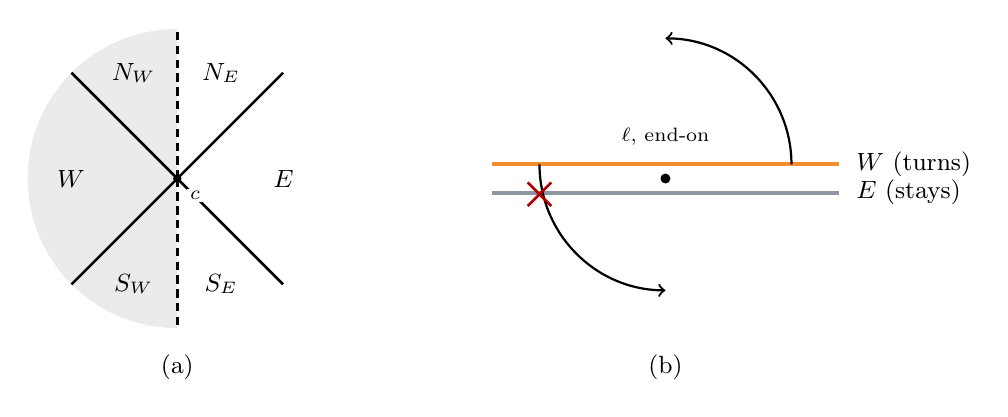
\begin{tikzpicture}[x=1cm,y=1cm,font=\small]
\begin{scope}
\fill[black!8] (0,0) -- (90:1.9) arc (90:270:1.9) -- cycle;
\foreach \a in {45,135,225,315} \draw[line width=0.9pt] (0,0)--(\a:1.9);
\foreach \a in {90,270} \draw[line width=0.9pt,dash pattern=on 3pt off 2pt] (0,0)--(\a:1.9);
\node at (0:1.35) {$E$}; \node at (180:1.35) {$W$};
\node at (67.5:1.45) {$N_E$}; \node at (112.5:1.45) {$N_W$};
\node at (247.5:1.45) {$S_W$}; \node at (292.5:1.45) {$S_E$};
\fill (0,0) circle (1.5pt); \node[anchor=north west,font=\scriptsize,fill=white,inner sep=1pt] at (0.12,-0.12) {$c$};
\node at (0,-2.4) {(a)};
\end{scope}
\begin{scope}[xshift=6.2cm]
\draw[line width=1.4pt,cP1] (-2.2,0.18)--(2.2,0.18); \node[anchor=west] at (2.3,0.18) {$W$ (turns)};
\draw[line width=1.4pt,cA] (-2.2,-0.18)--(2.2,-0.18); \node[anchor=west] at (2.3,-0.18) {$E$ (stays)};
\fill (0,0) circle (1.8pt); \node[anchor=south,font=\scriptsize] at (0,0.3) {$\ell$, end-on};
\draw[->,line width=0.8pt] (-1.6,0.18) arc (180:270:1.6);
\draw[->,line width=0.8pt] (1.6,0.18) arc (0:90:1.6);
\draw[red!70!black,line width=1pt] (-1.75,-0.35)--(-1.45,-0.05) (-1.75,-0.05)--(-1.45,-0.35);
\node at (0,-2.4) {(b)};
\end{scope}
\end{tikzpicture}
\caption{(a) Around $c$ in resolution B, just before the vertical (dashed) is folded: the diagonals divide the paper into sectors $E,N,W,S$, and the vertical cuts $N$ and $S$ in half. The moving paper must be one whole side of the vertical, for instance the shaded one. (b) Cross-section through the stack, looking along $\ell$. The face $W$ turns over about $\ell$ while $E$ stays. Its two halves leave the plane in opposite directions, so one of them must pass through $E$ (cross).}
\label{fig:sector}
\end{figure}

With B excluded, the second pattern has a unique resolution, A. In folding terms: fold the sheet in half along $X$, fold the big V's and the small V's through both layers, then make the rectangle fold $R$, which erases the two ends of $X$. The order of Proposition~\ref{prop:deer} has $24$ linear extensions: $X$ first, $R$ last, and $U,L,V^+,V^-$ in any order.

Colour plays no part here. Every vertex satisfies Maekawa's theorem whichever reading is chosen, and the degree-four dichotomy of Section~\ref{sec:colour} does not apply at $c$, where six creases meet. What separates A from B is foldability. B would need a move that folds all three lines at $c$ at once, a collapse, which the single-line model excludes.

\section{Toward an algorithm}\label{sec:algo}

The analysis suggests a pipeline in which every step except the first is exact.
\begin{enumerate}
\item \emph{Discretize.} Find the coarsest unit $2\pi/N$ for which all directions are integral within tolerance. Bisection-based designs give $N$ a power of two.
\item \emph{Local stage.} At each interior vertex, enumerate the admissible pairs from~\eqref{eq:maps} and the perfect pairings, keeping those whose local order is acyclic. Vertex degrees are small, so enumeration is cheap; in the first example every pairing was forced.
\item \emph{Defects.} A vertex where no perfect pairing survives is a defect. This includes every vertex without a perfect pairing, like $\vstar$, and every vertex without a collinear pair, like $p_\pm$ in Section~\ref{sec:deer}. At a defect, find the directions in which a hidden pair would let every half-edge be paired with an acyclic local order, and trace each ray.
\item \emph{Global stage.} Choose hidden pairs and witnesses to satisfy acyclicity (O), and minimize the number of hidden pairs. This is a small constraint-satisfaction problem; in general it could be handed to a SAT or ILP solver.
\item \emph{Foldability.} If several resolutions remain, test each vertex where they differ for an order of its chains in which every fold passes the test of Proposition~\ref{prop:notB}: the switch between moving and staying paper falls exactly at the new creases, and no face turns over about the fold line while another face lying across it stays. The test is local and needs only the folding maps of the few sectors around the vertex.
\item \emph{Output} the chains and the Hasse diagram of the basic order.
\end{enumerate}

The examples also mark the limits.
\begin{itemize}
\item \emph{Assumption~\ref{ass:pairs}} fails for folds through points where several earlier creases meet. There a chain may have more than two half-edges, related by products of reflections, which form a dihedral group generated by the $\sigma_c$.
\item \emph{Symmetric vertices}, such as those in patterns built on a $45^\circ$ grid, can have many perfect pairings, so the local stage stops being forced. The foldability test removes some of them, as at the centre of the second example.
\item \emph{Collapse-style patterns}, folded all at once rather than in steps, need not decompose into chains at all. The foldability test assumes a single fold line per move. A vertex that was in fact collapsed in one motion would be misread, either as a cancelled crease (Lemma~\ref{lem:first}) or by rejecting a reading that only a collapse can produce, like B in Section~\ref{sec:deer}.
\item \emph{Hidden pairs} could in general also sit on top of a visible crease, with three creases summing to one. Without minimality the search space would be unbounded.
\item \emph{Right-angle crossings} carry no ordering information without colour (Section~\ref{sec:colour}).
\end{itemize}

Related work. Deciding whether a crease pattern can be folded flat at all is NP-hard~\cite{bernhayes}; see~\cite{demaine} for background. Akitaya, Mitani, Kanamori and Fukui~\cite{akitaya} recover folding sequences by graph rewriting with a library of standard moves. Their notion of mirror-image crease pairs requires opposite colours. In our example six chains, the $P_i^{\pm}$, keep a single colour through every bend, so only a colour-blind pairing finds them.

\begin{thebibliography}{9}
\bibitem{akitaya} H.~A. Akitaya, J.~Mitani, Y.~Kanamori, Y.~Fukui, Generating folding sequences from crease patterns of flat-foldable origami, \emph{ACM SIGGRAPH 2013 Posters}.
\bibitem{bernhayes} M.~Bern, B.~Hayes, The complexity of flat origami, \emph{Proc.\ 7th ACM--SIAM Symposium on Discrete Algorithms} (1996), 175--183.
\bibitem{demaine} E.~D. Demaine, J.~O'Rourke, \emph{Geometric Folding Algorithms: Linkages, Origami, Polyhedra}, Cambridge University Press, 2007.
\bibitem{hull} T.~Hull, On the mathematics of flat origamis, \emph{Congressus Numerantium} 100 (1994), 215--224.
\end{thebibliography}

\appendix
\section{All interior vertices}\label{app:table}

For each interior vertex, the table gives approximate coordinates, the direction multiset $D_v$ in units of $\pi/32$, and the unique perfect pairing. Each pair is written with its chain name and its type: $\tau$ for straight, $\sigma_c$ for reflected with witness line of direction $c\bmod 32$, and $\tau{=}\sigma_c$ where the pair is straight and also crosses the line $c$ at a right angle. At the starred vertex $\vstar$, $\bar 0$ denotes the two hidden half-edges. The table, Table~\ref{tab:chains}, the order of Section~\ref{sec:order} and the count of linear extensions were generated by the accompanying script \texttt{reflection\_analysis.py}, which reads crease patterns in the FOLD format, from the coordinates of the crease pattern, using only the integer arithmetic of Section~\ref{sec:discrete} after the initial rounding of directions.

{\small
\begin{longtable}{lll}
\toprule
vertex & $D_v$ & pairing\\
\midrule
\endhead
(4, 6.343) & $4,10,16,36,56,62$ & $P_1^{+}\!:\{4,36\}\,\tau$; $C'\!:\{10,62\}\,\sigma_{4}$; $C\!:\{16,56\}\,\sigma_{4}$ \\
(1.313, 6) & $0,16,32,48$ & $A^{+}\!:\{0,32\}\,\tau{=}\sigma_{16}$; $E\!:\{16,48\}\,\tau{=}\sigma_{0}$ \\
(1.92, 6) & $0,19,32,45$ & $A^{+}\!:\{0,32\}\,\tau$; $E'\!:\{19,45\}\,\sigma_{0}$ \\
(3.172, 6) & $0,4,32,60$ & $A^{+}\!:\{0,32\}\,\tau$; $P_1^{+}\!:\{4,60\}\,\sigma_{0}$ \\
(4.343, 6) & $0,24,32,40$ & $A^{+}\!:\{0,32\}\,\tau$; $C\!:\{24,40\}\,\sigma_{0}$ \\
(5.725, 6) & $0,30,32,34$ & $A^{+}\!:\{0,32\}\,\tau$; $C'\!:\{30,34\}\,\sigma_{0}$ \\
(6, 6) & $0,8,32,56$ & $A^{+}\!:\{0,32\}\,\tau$; $P_2^{+}\!:\{8,56\}\,\sigma_{0}$ \\
(7.172, 6) & $0,12,32,52$ & $A^{+}\!:\{0,32\}\,\tau$; $P_3^{+}\!:\{12,52\}\,\sigma_{0}$ \\
(7.293, 5.707) & $4,20,36,52$ & $I\!:\{4,36\}\,\tau{=}\sigma_{20}$; $P_3^{+}\!:\{20,52\}\,\tau{=}\sigma_{4}$ \\
(4, 5.657) & $2,8,28,48,54,60$ & $C'\!:\{2,54\}\,\sigma_{28}$; $C\!:\{8,48\}\,\sigma_{28}$; $P_1^{+}\!:\{28,60\}\,\tau$ \\
(6.586, 5.414) & $4,24,44,56$ & $I\!:\{4,44\}\,\sigma_{24}$; $P_2^{+}\!:\{24,56\}\,\tau$ \\
(6.293, 4.707) & $12,28,44,60$ & $I\!:\{12,44\}\,\tau{=}\sigma_{28}$; $P_1^{+}\!:\{28,60\}\,\tau{=}\sigma_{12}$ \\
(1.313, 4) & $0,13,16,32,48,51$ & $A^{0}\!:\{0,32\}\,\tau{=}\sigma_{16}$; $E'\!:\{13,51\}\,\sigma_{0}$; $E\!:\{16,48\}\,\tau{=}\sigma_{0}$ \\
(4, 4) & $0,16,32,48$ & $A^{0}\!:\{0,32\}\,\tau{=}\sigma_{16}$; $C\!:\{16,48\}\,\tau{=}\sigma_{0}$ \\
(5.107, 4) & $0,22,32,42$ & $A^{0}\!:\{0,32\}\,\tau$; $C'\!:\{22,42\}\,\sigma_{0}$ \\
(6, 4)$^{\ast}$ & $12,32,40,52,\bar 0,\bar 0$ & $I\!:\{12,52\}\,\sigma_{0}$; $A^{0}\!:\{32,\bar 0\}\,\tau$; $F\!:\{40,\bar 0\}\,\sigma_{20}$ \\
(6.293, 3.293) & $4,20,36,52$ & $P_1^{-}\!:\{4,36\}\,\tau{=}\sigma_{20}$; $I\!:\{20,52\}\,\tau{=}\sigma_{4}$ \\
(4.586, 2.586) & $0,4,8,36$ & $F\!:\{0,8\}\,\sigma_{4}$; $P_1^{-}\!:\{4,36\}\,\tau$ \\
(6.586, 2.586) & $8,20,32,40,48,60$ & $P_2^{-}\!:\{8,40\}\,\tau$; $I\!:\{20,60\}\,\sigma_{8}$; $F\!:\{32,48\}\,\sigma_{8}$ \\
(4, 2.343) & $4,10,16,36,56,62$ & $P_1^{-}\!:\{4,36\}\,\tau$; $C'\!:\{10,62\}\,\sigma_{4}$; $C\!:\{16,56\}\,\sigma_{4}$ \\
(7.293, 2.293) & $12,28,44,60$ & $P_3^{-}\!:\{12,44\}\,\tau{=}\sigma_{28}$; $I\!:\{28,60\}\,\tau{=}\sigma_{12}$ \\
(1.313, 2) & $0,16,32,48$ & $A^{-}\!:\{0,32\}\,\tau{=}\sigma_{16}$; $E\!:\{16,48\}\,\tau{=}\sigma_{0}$ \\
(1.92, 2) & $0,19,32,45$ & $A^{-}\!:\{0,32\}\,\tau$; $E'\!:\{19,45\}\,\sigma_{0}$ \\
(3.172, 2) & $0,4,32,60$ & $A^{-}\!:\{0,32\}\,\tau$; $P_1^{-}\!:\{4,60\}\,\sigma_{0}$ \\
(4.343, 2) & $0,24,32,40$ & $A^{-}\!:\{0,32\}\,\tau$; $C\!:\{24,40\}\,\sigma_{0}$ \\
(5.725, 2) & $0,30,32,34$ & $A^{-}\!:\{0,32\}\,\tau$; $C'\!:\{30,34\}\,\sigma_{0}$ \\
(6, 2) & $0,8,32,56$ & $A^{-}\!:\{0,32\}\,\tau$; $P_2^{-}\!:\{8,56\}\,\sigma_{0}$ \\
(6.586, 2) & $0,16,32,48$ & $A^{-}\!:\{0,32\}\,\tau{=}\sigma_{16}$; $F\!:\{16,48\}\,\tau{=}\sigma_{0}$ \\
(7.172, 2) & $0,12,32,52$ & $A^{-}\!:\{0,32\}\,\tau$; $P_3^{-}\!:\{12,52\}\,\sigma_{0}$ \\
(4, 1.657) & $2,8,28,48,54,60$ & $C'\!:\{2,54\}\,\sigma_{28}$; $C\!:\{8,48\}\,\sigma_{28}$; $P_1^{-}\!:\{28,60\}\,\tau$ \\
(4.586, 1.414) & $0,28,56,60$ & $F\!:\{0,56\}\,\sigma_{28}$; $P_1^{-}\!:\{28,60\}\,\tau$ \\
(6.586, 1.414) & $16,24,32,56$ & $F\!:\{16,32\}\,\sigma_{24}$; $P_2^{-}\!:\{24,56\}\,\tau$ \\
\bottomrule
\end{longtable}}

\end{document}
